\documentclass[tikz,border=4pt]{standalone}
\usepackage{amsmath}
\usetikzlibrary{arrows.meta,positioning}
\begin{document}
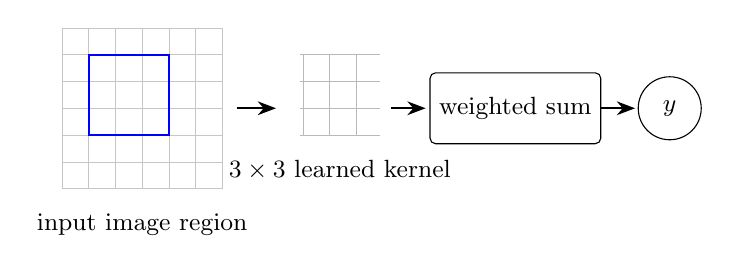
\begin{tikzpicture}[
  >=Stealth,
  every node/.style={font=\small},
  box/.style={draw,rounded corners=2pt,minimum height=9mm,align=center},
  arrow/.style={->,thick}
]
  \draw[step=0.34cm,gray!45,very thin] (0,0) grid (2.04,2.04);
  \draw[blue,thick] (0.34,0.68) rectangle (1.36,1.70);
  \node[below=2mm] at (1.02,0) {input image region};
  \draw[arrow] (2.22,1.02) -- (2.72,1.02);
  \draw[step=0.34cm,gray!55,very thin] (3.02,0.68) grid (4.04,1.70);
  \node[below=2mm] at (3.53,0.68) {$3\times3$ learned kernel};
  \draw[arrow] (4.18,1.02) -- (4.62,1.02);
  \node[box,minimum width=2.15cm] (sum) at (5.76,1.02) {weighted sum};
  \draw[arrow] (6.85,1.02) -- (7.28,1.02);
  \node[draw,circle,minimum size=8mm] at (7.72,1.02) {$y$};
\end{tikzpicture}
\end{document}
